\chapter{Modeling of Short-term Mechanism of Arterial Pressure Control in the Cardiovascular System: Object-oriented and Acausal Approach}\label{app:modeling}
The paper \cite{Kulhanek2014Modeling} published as
 
\bibentry{Kulhanek2014Modeling}

Available online at \url{http://dx.doi.org/10.1016/j.compbiomed.2014.08.025}

The author of this thesis contributed to the idea of building complex mathematical models from the basic components and keeping them in an understandable and maintainable form. Additionally, the author implemented several basic blocks and models of a pulsatile cardiovascular system in Modelica language. The other co-authors implemented the library in order to model physiology, using an integrative approach. They also implemented the complex models, which integrated different domains together.
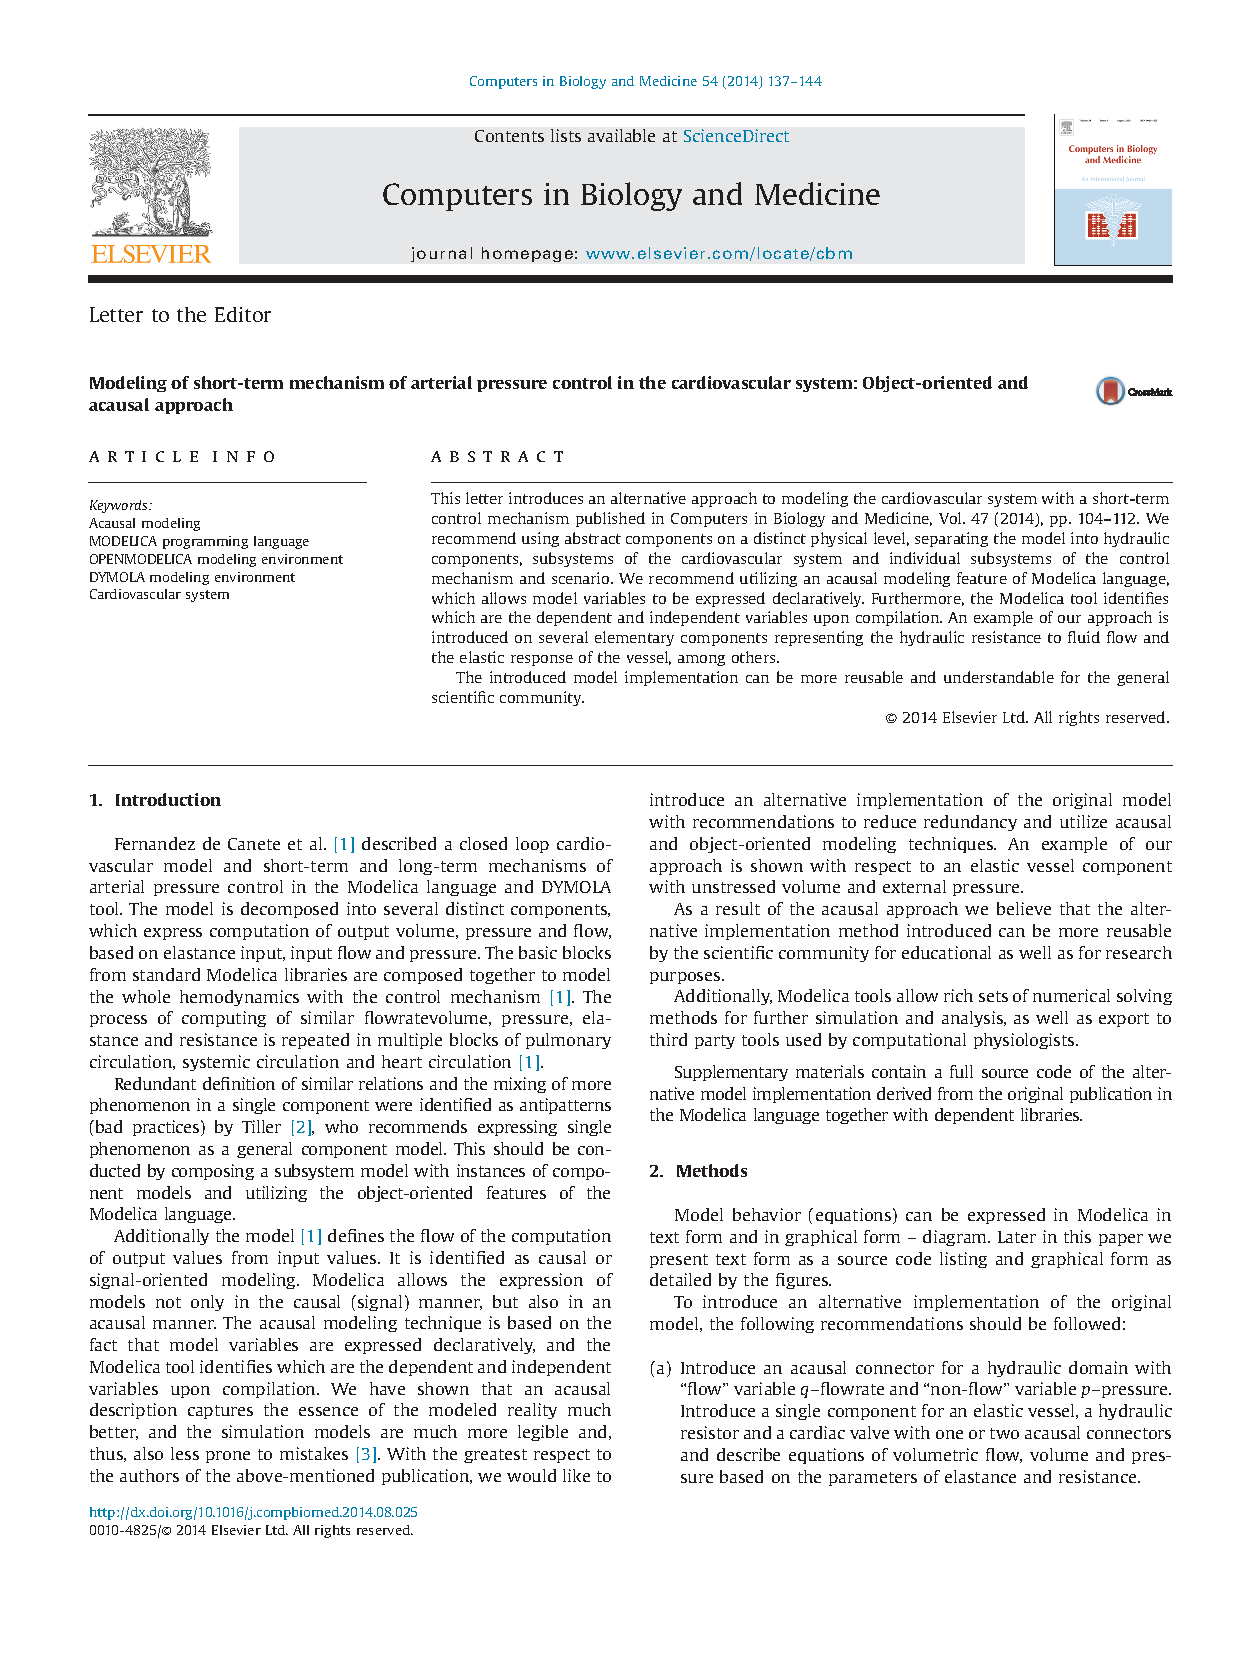
\includepdf[scale=0.9,pages={-},pagecommand={\thispagestyle{plain}}]{appendix/LetterToEditorNew2.pdf}
